\section{Langkawi}

17 mai 2008

\begin{multicols}{2}

Aujourd'hui au programme, les iles Langkawi où je suis actuellement. Il s'agit des dernières îles malaisiennes avant la Thaïlande, c'est donc ici que nous feront tamponner nos passeports avant de remonter. Nous sommes arrivés au Sud et avons dormis une nuit au mouillage dans une petite crique bien sympa.

%<div><object width="640" height="505"><param name="movie" value="http://www.dailymotion.com/swf/x5lrr0&related=1"></param><param name="allowFullScreen" value="true"></param><param name="allowScriptAccess" value="always"></param><embed src="http://www.dailymotion.com/swf/x5lrr0&related=1" type="application/x-shockwave-flash" width="640" height="505" allowFullScreen="true" allowScriptAccess="always"></embed></object></div>

Puis c'est reparti on remonte un peu au nord pour aller dans une marina, on compte rester quelques jours ici. Et là je dois le dire, car c'est assez rare pour être souligné, même Patrick a été impressionné par la beauté de l'endroit (oui, on a pas tous la chance d'avoir vécu en Calédonie). L'entrée de la marina est tout simplement superbe.

%\hspace*{-0.65cm}
%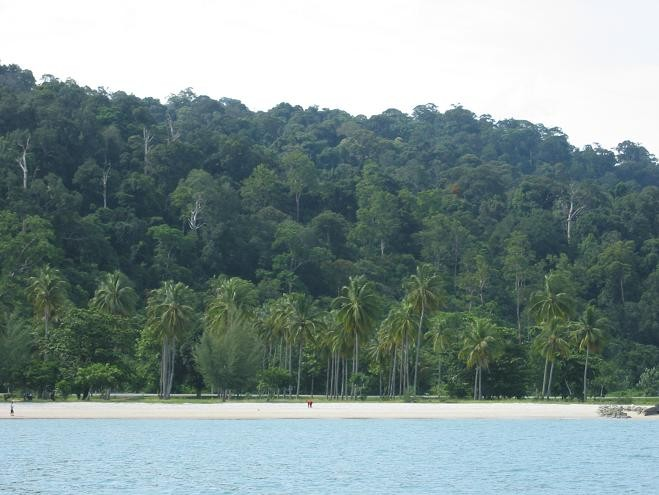
\includegraphics[width=4.8cm]{articles/langkawi/1211018197eneE.jpg}
%Plage de Langkawi.

%\hspace*{-0.65cm}
%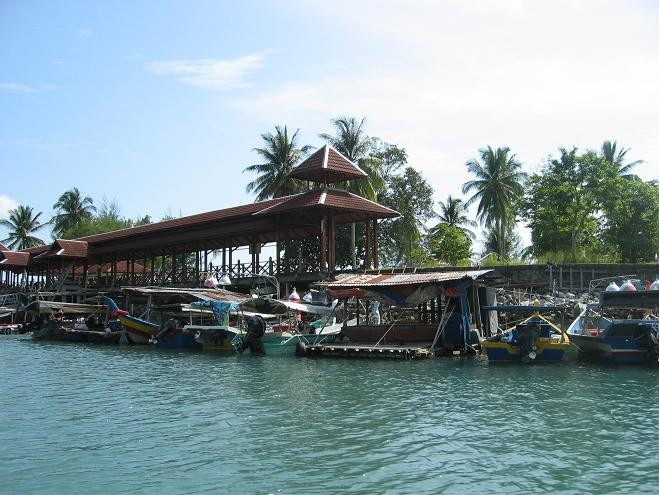
\includegraphics[width=4.8cm]{articles/langkawi/1211018204F7Ee.jpg}
%Entrée de la marina.

%\hspace*{-0.65cm}
%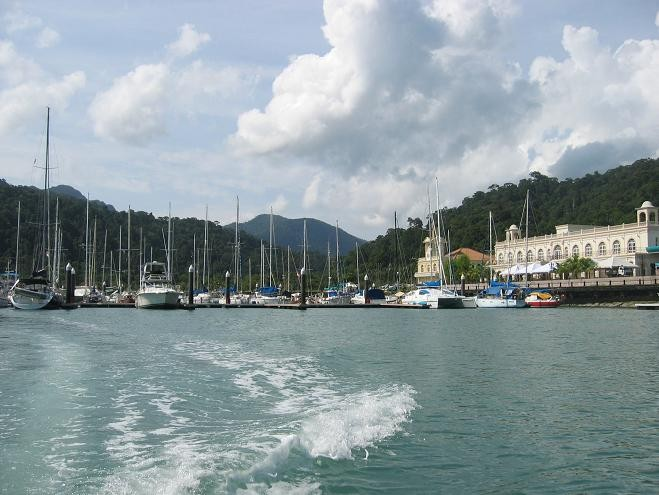
\includegraphics[width=4.8cm]{articles/langkawi/1211018457DniB.jpg}
%Ben... sortie de la marina... le même endroit, quoi.

Et c'est parti pour visiter, pas loin de la marina il y a des chutes d'eau. On voulait au depart aller prendre un télépherique qui monte au sommet de la colline pour voir toute l'île mais il était en réparation, ce n'est que partie remise.

%\hspace*{-0.65cm}
%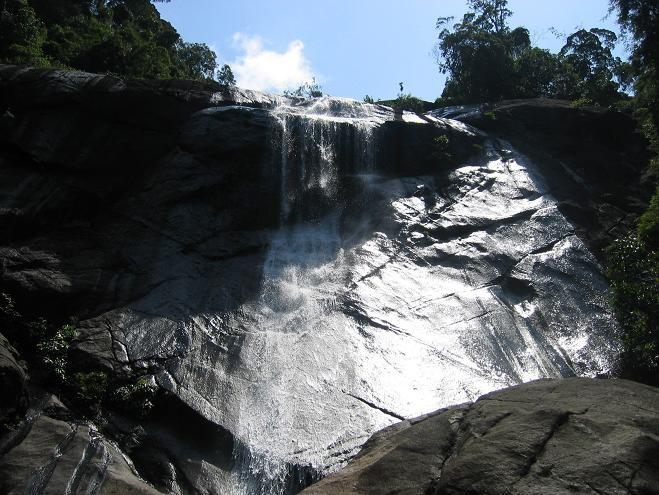
\includegraphics[width=4.8cm]{articles/langkawi/1211018190Pmip.jpg}
%Cascade.

Je complèterai cet article dans les jours qui viennent avec des photos du tour de l'île, je vais louer un scooter car il parait que ça vaut vraiment le coup a faire...

Je vous laisse sur une petite note poissonistique.

%<div><object width="640" height="505"><param name="movie" value="http://www.dailymotion.com/swf/x5gab6&v3=1&related=1"></param><param name="allowFullScreen" value="true"></param><param name="allowScriptAccess" value="always"></param><embed src="http://www.dailymotion.com/swf/x5gab6&v3=1&related=1" type="application/x-shockwave-flash" width="640" height="505" allowFullScreen="true" allowScriptAccess="always"></embed></object></div>

Voici comme promis quelques photos en plus.

%\hspace*{-0.65cm}
%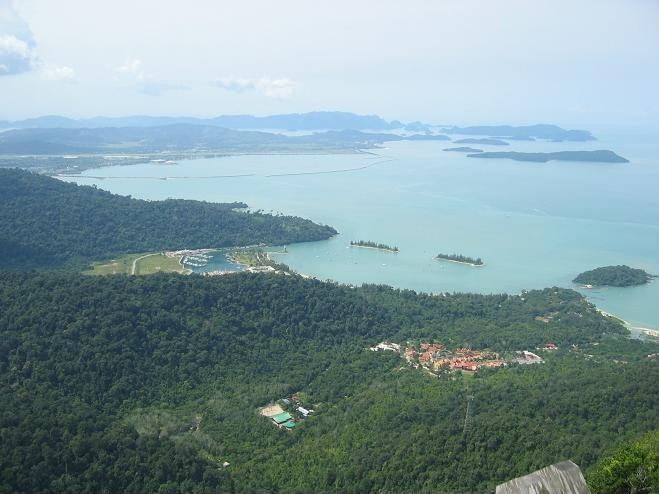
\includegraphics[width=4.8cm]{articles/langkawi/1212397933wQ6v.jpg}
%La marina vue d'en haut.

%\hspace*{-0.65cm}
%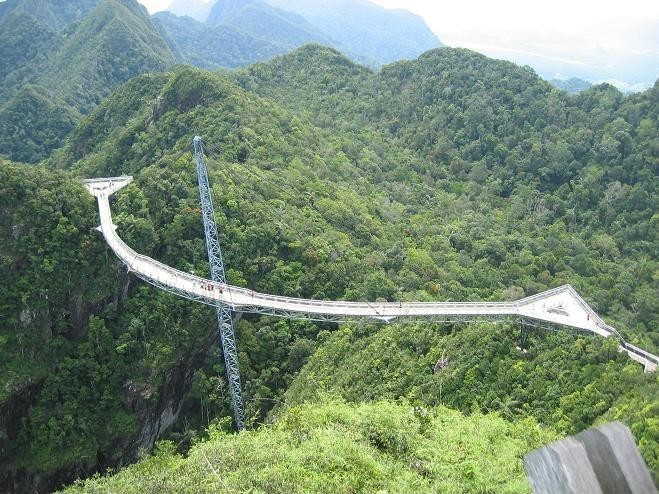
\includegraphics[width=4.8cm]{articles/langkawi/1212398042f2k1.jpg}
%Une passerelle touristique.

%\hspace*{-0.65cm}
%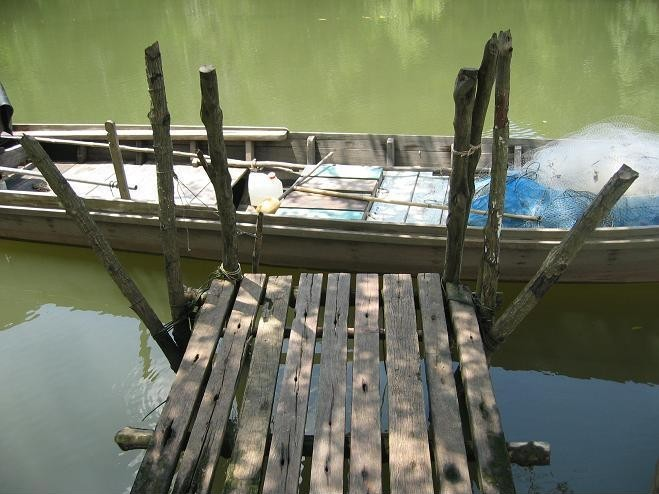
\includegraphics[width=4.8cm]{articles/langkawi/1212397931akoQ.jpg}
%Petit ponton dans la mangrove.

\end{multicols}

\bigskip
\textbf{\textsc{Commentaires}}

\medskip
Titou a écrit le 18 mai 2008 :
\begin{displayquote}
Je me répète\dots mais on ne gère pas tous l'addition :p ! Attand on est qu'à l'UTBM, ça fait partie du programme de dernière année  et y en a qui n'y son pas encore\dots
Allez enjoy and take care. Biz ma poule.
\end{displayquote}

\medskip
Peggy a écrit le 19 mai 2008 :
\begin{displayquote}
ETIENNE LE JUSTICIER (des petits poissons)!!
Je me demande ce qu'il se passerait si tu sautais à l'eau, ils essayeraient de te grignoter les fesses peut être?
Bon, je sors!
Avant\dots petite réflexion 7+1=? (heureusement que les calculs restent simples!)
\end{displayquote}

\medskip
Etienne a écrit le 20 mai 2008 :
\begin{displayquote}
Y en a un qui m'a gniaqué le doigt, j'avais posé un bout de pain dessus et approché de l'eau car ce sont des poissons cracheurs, ils visent le bout de pain et le font tomber pour le récupérer. Seulement celui-ci m'a mordu le doigt, le suivant a mis un coup de boule dans le pain pour le faire tomber.
\end{displayquote}

\medskip
Pierre a écrit le 26 mai 2008 :
\begin{displayquote}
Hey!
C'est vrai que la plage est blasante\dots j'ai connu mieux!!!
Non sérieusement ça fait halluciner!
Continue de vendre du rêve!
Gad m'a rappelé : je lui ai proposé de te laisser un message sur ton blog\dots
Biz à toi.
\end{displayquote}

\medskip
Titou a écrit le 26 mai 2008 :
\begin{displayquote}
ON VEUT LA SUITE ! ON VEUT LA SUITE !
A BIENTOT TI DUD !
\end{displayquote}

\medskip
Tite soeur a écrit le 28 mai 2008 :
\begin{displayquote}
Pour moi, 4+8=12\dots ça reste simple\dots
On est le 28, et pas de nouvelle depuis le 20\dots va falloir penser à ceux qui restent en France et qui commencent à s'inquéter\dots
Donne nous des news\dots
A bientôt ti frère
Bisou.
\end{displayquote}

\vfill

